\documentclass[a4paper,11pt]{article}

\usepackage[french]{babel}
\usepackage[T1]{fontenc}
\usepackage[utf8]{inputenc}
\usepackage{lmodern}
\usepackage{microtype}

\usepackage{graphicx}
\graphicspath{ {./} }
\usepackage{hyperref}
\usepackage[margin=1in]{geometry} %Change la marge
\usepackage{xurl}

\date{}
\title{TIPE : Mis à jour du projet et avancées}
\author{DE CARVALHO Enzo et ALEXANDRINE Pedro}

\begin{document}
\maketitle
\section{Motivations : rappels}
	Le but est de modéliser, à l'aide de machine learning, l'évolution des 
	chiffres liès (à priori ici, les décès) et si possible, d'affiner la 			modélisation pour mieux prédir l'évolution de la courbe, et/ou étudier 			les limites de la modélisation

\section{Résultats et avancées actuelles}
	Nous avons alors, dans un premier lieu réalisé différentes regressions
	linéaire à l'aide du package \texttt{sklearn} en python proposant déjà
	quelques régresseurs linéaire classiques, ainsi qu'une prédiction
	faite avec le modèle Prophet.
	Toutes les prédictions sont faîtes sur la base de données :
	\url{https://github.com/opencovid19-fr/data}\\
	\begin{itemize}
		\item Modèle ElasticNet (prédit les données entre le 02/12/20 et 16/12/20)\\
		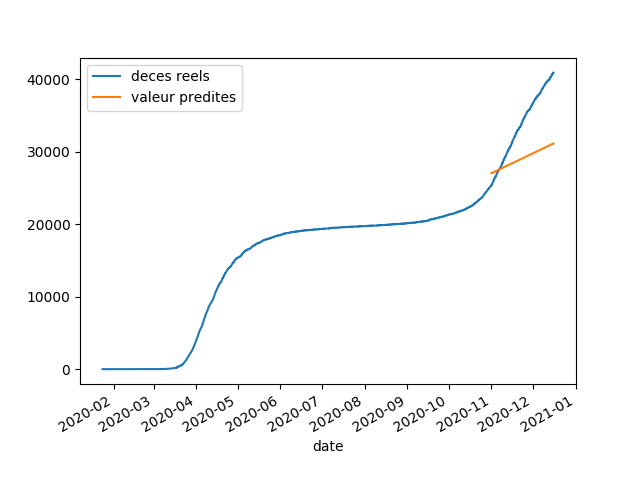
\includegraphics[scale=1]{Figure_EN}\\

		\item Modèle SVR (prédit les données entre le 02/12/20 et 16/12/20)\\
		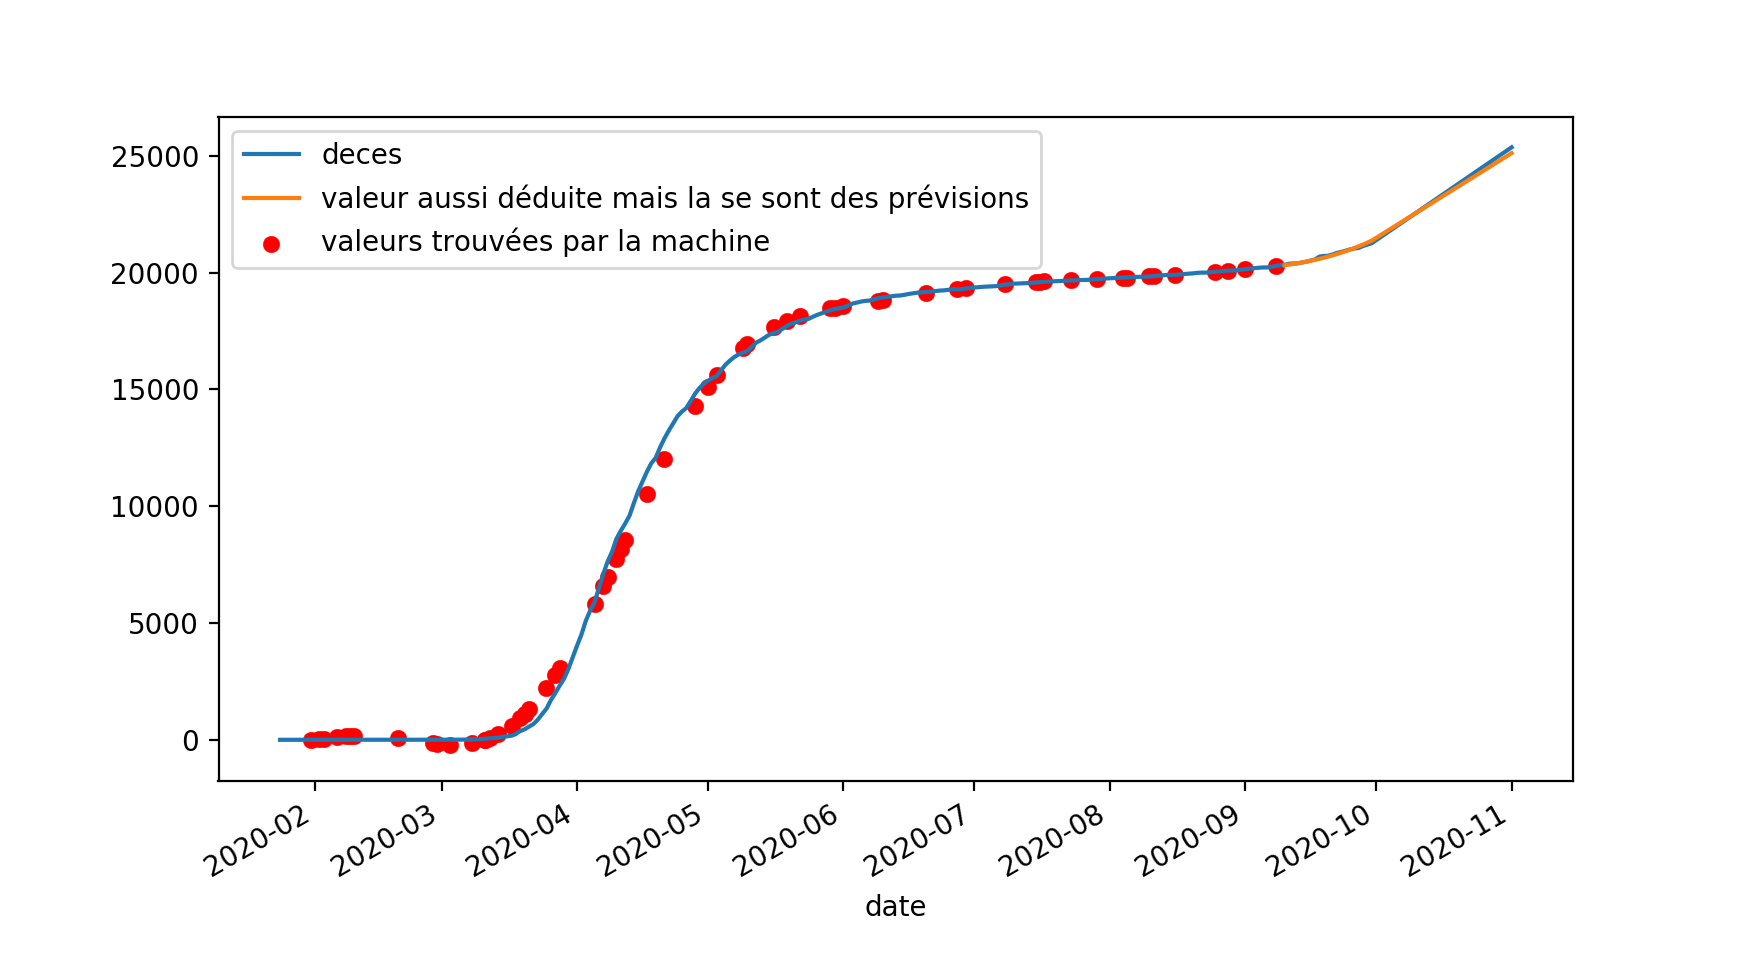
\includegraphics[scale=0.7]{Figure_SVR}\\
		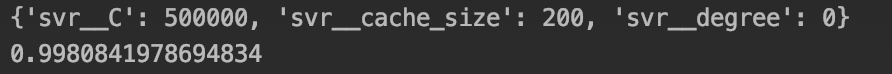
\includegraphics[scale=1]{params}\\
		
		\item Modèle Prophet(prédit les données entre le 06/12/20 et 29/12/20)\\
		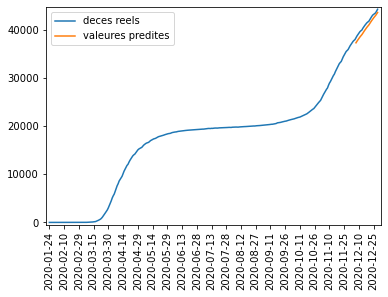
\includegraphics[scale=1]{Figure_Prophet}\\
		
	\end{itemize}

\section{Overture possible}
	La suite logique dans notre programme de "expérimentation de
	regression" serait alors d'aller au délà de la simple régression
	linéaire.
	Pour cela, quelques pistes sont envisageable, même si celle ci ne
	remette pas en question la direction actuelle de notre TIPE.
	Elles sont :
	\begin{itemize}
		\item méthode de Levenberg-Marquardt :\\ 
		\url{https://fr.wikipedia.org/wiki/Algorithme_de_Levenberg-Marquardt}
		\item méthode ARMA
	\end{itemize}
\end{document}